\documentclass[border=4pt]{standalone}
\usepackage{amsmath,amssymb,bm}
\usepackage{tikz}
\usetikzlibrary{positioning,arrows.meta,calc,fit,backgrounds}
\newcommand{\btheta}{\bm\theta}\newcommand{\bs}{\boldsymbol}
\definecolor{cPDE}{HTML}{3E5C8A}\definecolor{fPDE}{HTML}{EAEFF7}
\definecolor{cTR}{HTML}{A0522D}\definecolor{fTR}{HTML}{F7EFE6}
\definecolor{cNN}{HTML}{2E7D5B}\definecolor{fNN}{HTML}{E6F2EC}
\definecolor{cRT}{HTML}{555555}\definecolor{fRT}{HTML}{F1F1F3}
\tikzset{
  box/.style={draw,rounded corners=2pt,line width=0.6pt,align=center,inner sep=4pt,minimum height=1.25cm,font=\small},
  pde/.style={box,draw=cPDE,fill=fPDE},
  tr/.style={box,draw=cTR,fill=fTR},
  nn/.style={box,draw=cNN,fill=fNN},
  rt/.style={box,draw=cRT,fill=fRT},
  arr/.style={-{Stealth[length=5pt]},line width=0.6pt,draw=black!65},
  lab/.style={font=\scriptsize,above,midway},
  neuron/.style={circle,draw=cNN!85!black,fill=white,line width=0.55pt,inner sep=0pt},
  inode/.style={neuron,minimum size=0.46cm,font=\small,text=cNN!65!black},
  hnode/.style={neuron,minimum size=0.57cm,path picture={
    \begin{scope}[shift={(path picture bounding box.center)},line cap=round]
      \draw[black!35,line width=0.28pt] (-0.21,0)--(0.21,0) (0,-0.17)--(0,0.17);
      \draw[cTR!85!black,line width=0.9pt]
        (-0.20,-0.115) .. controls (-0.06,-0.115) and (-0.065,-0.095) .. (0,0)
                       .. controls (0.065,0.095) and (0.06,0.115) .. (0.20,0.115);
    \end{scope}}},
  onode/.style={circle,fill=cNN!78!black,minimum size=0.21cm,inner sep=0pt},
  wire/.style={draw=cNN!43,line width=0.36pt},
  stage/.style={font=\bfseries\large,text=black!70,rotate=90}
}
\begin{document}
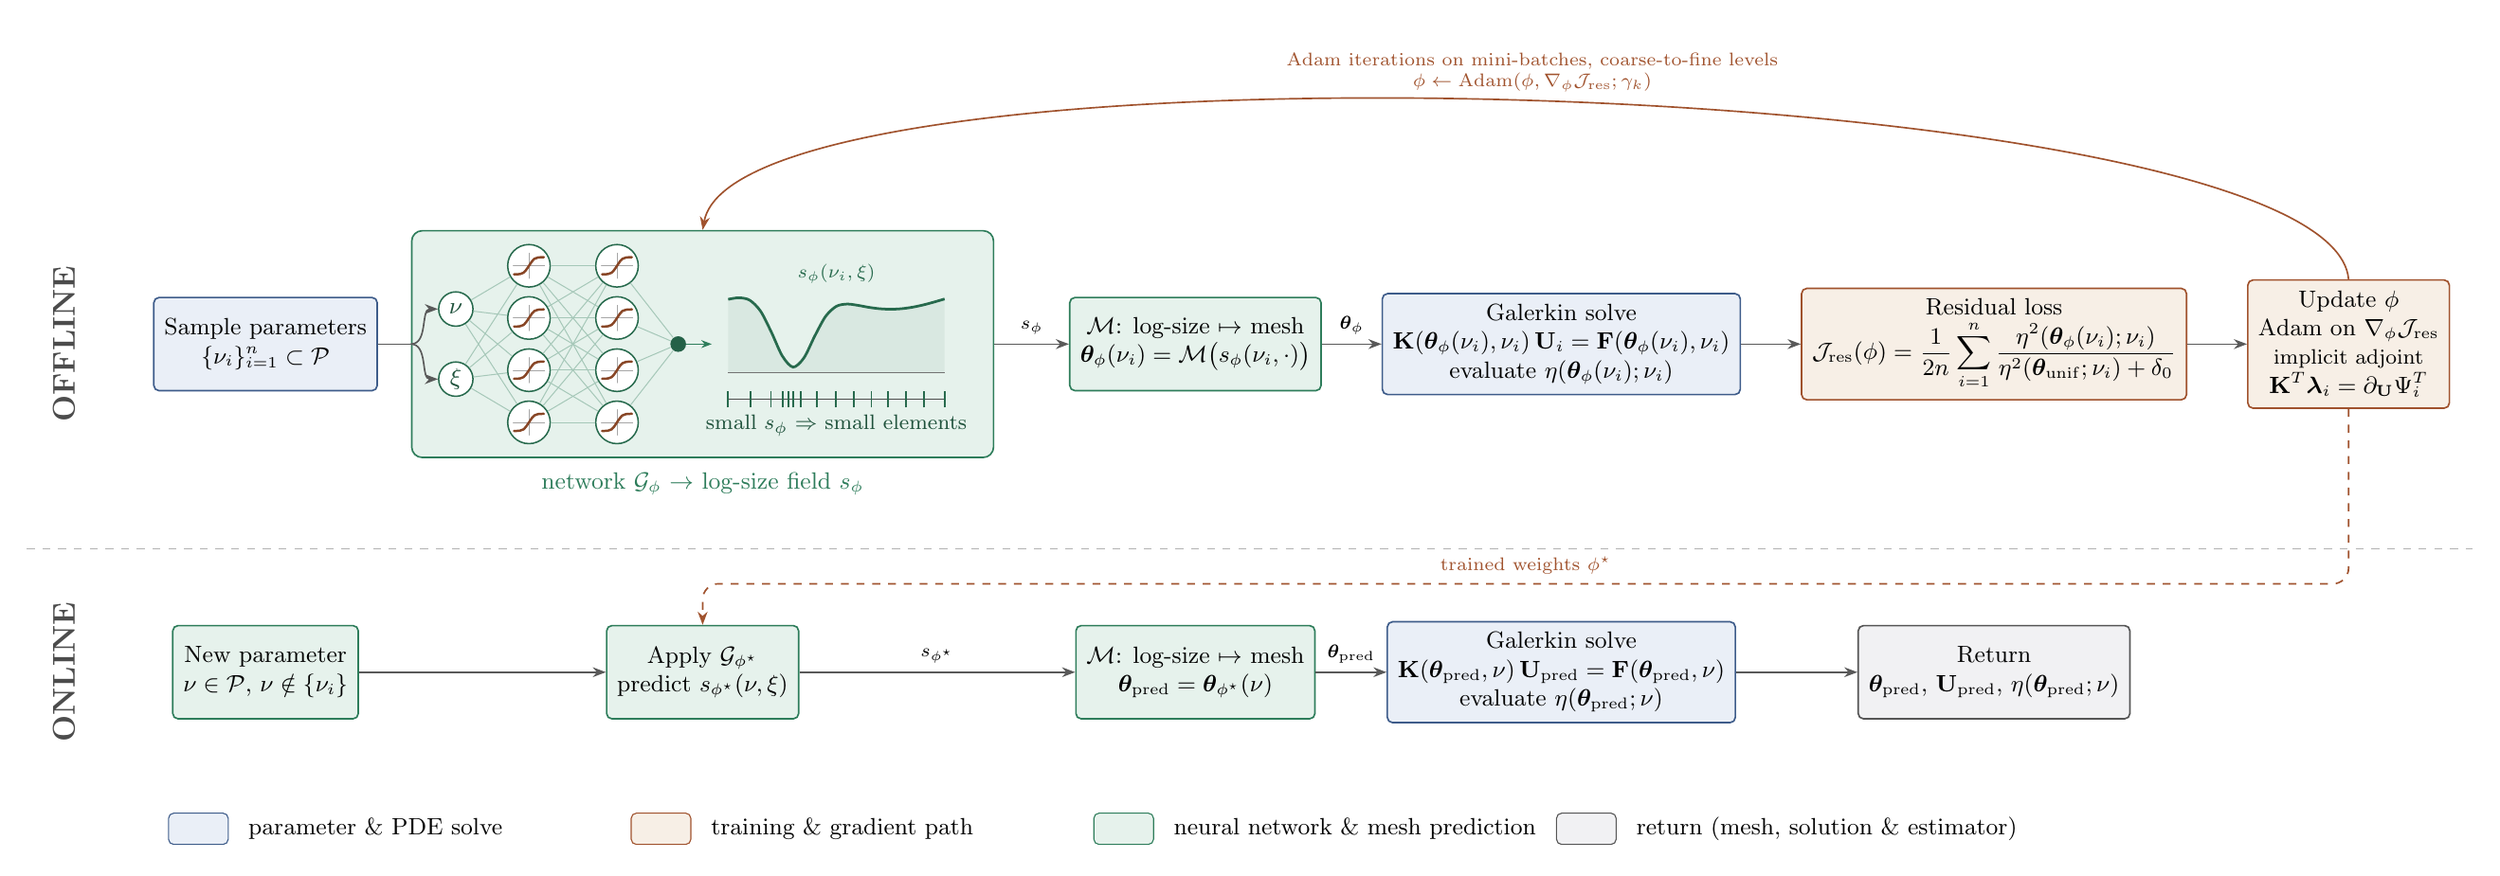
\begin{tikzpicture}[node distance=0.75cm]
% ---------------- OFFLINE ----------------
\node[stage] at (-1.4,0) {OFFLINE};
\node[pde] (samp) at (1.3,0) {Sample parameters\\ $\{\nu_i\}_{i=1}^{n}\subset\mathcal P$};
\begin{scope}[shift={(3.85,0)}]
  \node[inode] (xn) at (0,0.47) {$\nu$};
  \node[inode] (xx) at (0,-0.47) {$\xi$};
  \foreach \y [count=\i] in {1.05,0.35,-0.35,-1.05}{
    \node[hnode] (a\i) at (0.98,\y) {};
    \node[hnode] (b\i) at (2.16,\y) {};
  }
  \node[onode] (o) at (2.98,0) {};
  \foreach \s in {xn,xx}{\foreach \i in {1,...,4}{\draw[wire] (\s)--(a\i);}}
  \foreach \i in {1,...,4}{\foreach \j in {1,...,4}{\draw[wire] (a\i)--(b\j);}}
  \foreach \j in {1,...,4}{\draw[wire] (b\j)--(o);}
  \draw[-{Stealth[length=4pt]},cNN,line width=0.6pt] (o.east)--(3.43,0);
  % inset: log-size field and the mesh it induces
  \begin{scope}[shift={(3.65,0.22)},x=2.9cm,y=0.55cm]
    \fill[cNN!18] (0,-1.1) -- plot[smooth] coordinates {(0.000,0.691) (0.050,0.730) (0.100,0.669) (0.150,0.400) (0.200,-0.114) (0.250,-0.689) (0.300,-0.962) (0.350,-0.736) (0.400,-0.204) (0.450,0.275) (0.500,0.522) (0.550,0.576) (0.600,0.544) (0.650,0.496) (0.700,0.462) (0.750,0.450) (0.800,0.462) (0.850,0.498) (0.900,0.553) (0.950,0.623) (1.000,0.700)} -- (1,-1.1) -- cycle;
    \draw[cNN!85!black,line width=1.0pt] plot[smooth] coordinates {(0.000,0.691) (0.050,0.730) (0.100,0.669) (0.150,0.400) (0.200,-0.114) (0.250,-0.689) (0.300,-0.962) (0.350,-0.736) (0.400,-0.204) (0.450,0.275) (0.500,0.522) (0.550,0.576) (0.600,0.544) (0.650,0.496) (0.700,0.462) (0.750,0.450) (0.800,0.462) (0.850,0.498) (0.900,0.553) (0.950,0.623) (1.000,0.700)};
    \draw[black!55,line width=0.4pt] (0,-1.1)--(1,-1.1);
    \node[font=\scriptsize,text=cNN!85!black,anchor=south] (slab) at (0.5,0.85) {$s_\phi(\nu_i,\xi)$};
    \draw[black!70,line width=0.5pt] (0,-1.75)--(1,-1.75);
    \foreach \k in {0.0000,0.1027,0.1975,0.2542,0.2792,0.2990,0.3364,0.4084,0.4967,0.5817,0.6616,0.7396,0.8196,0.9053,1.0000}{\draw[cNN!85!black,line width=0.7pt] (\k,-1.95)--(\k,-1.55);}
    \node[anchor=north,inner sep=0pt,font=\footnotesize,text=cNN!65!black]
      (meshlabel) at (0.5,-2.12) {small $s_\phi$ $\Rightarrow$ small elements};
    \coordinate (insetNE) at (1,1.2);
  \end{scope}
\end{scope}
\begin{scope}[on background layer]
  \node[draw=cNN,fill=fNN,rounded corners=4pt,line width=0.6pt,
    fit=(xn)(xx)(a1)(a4)(o)(slab)(meshlabel)(insetNE),inner xsep=10pt,inner ysep=5pt] (net) {};
\end{scope}
\node[font=\small,text=cNN,below=2pt of net] {network $\mathcal G_\phi$ $\to$ log-size field $s_\phi$};
\coordinate (split) at ($(samp.east)!0.55!(xn.west |- samp.east)$);
\draw[line width=0.6pt,draw=black!65] (samp.east)--(split);
\draw[arr] (split) to[out=0,in=180] (xn.west);
\draw[arr] (split) to[out=0,in=180] (xx.west);
\node[nn,right=1.0cm of net] (map) {$\mathcal M$: log-size $\mapsto$ mesh\\ $\btheta_\phi(\nu_i)=\mathcal M\bigl(s_\phi(\nu_i,\cdot)\bigr)$};
\draw[arr] (net)--node[lab]{$s_\phi$}(map);
\node[pde,right=0.8cm of map] (gal) {Galerkin solve\\ $\mathbf K(\btheta_\phi(\nu_i),\nu_i)\,\mathbf U_i=\mathbf F(\btheta_\phi(\nu_i),\nu_i)$\\ evaluate $\eta(\btheta_\phi(\nu_i);\nu_i)$};
\draw[arr] (map)--node[lab]{$\btheta_\phi$}(gal);
\node[tr,right=0.8cm of gal] (loss) {Residual loss\\[1pt] $\displaystyle\mathcal J_{\rm res}(\phi)=\frac1{2n}\sum_{i=1}^{n}\frac{\eta^2(\btheta_\phi(\nu_i);\nu_i)}{\eta^2(\btheta_{\rm unif};\nu_i)+\delta_0}$};
\draw[arr] (gal)--(loss);
\node[tr,right=0.8cm of loss] (upd) {Update $\phi$\\ Adam on $\nabla_\phi\mathcal J_{\rm res}$\\ \footnotesize implicit adjoint\\ $\mathbf K^{T}\bs\lambda_i=\partial_{\mathbf U}\Psi_i^{T}$};
\draw[arr] (loss)--(upd);
\draw[arr,draw=cTR] (upd.north) to[out=95,in=80,looseness=0.32] node[pos=0.5,above,font=\scriptsize,text=cTR,align=center]{Adam iterations on mini-batches, coarse-to-fine levels\\ $\phi\gets\operatorname{Adam}(\phi,\nabla_\phi\mathcal J_{\rm res};\gamma_k)$} (net.north);
% ---------------- separator ----------------
\draw[dashed,black!30] (-1.9,-2.75)--($(upd.east |- 0,-2.75)+(0.3,0)$);
% ---------------- ONLINE ----------------
\node[stage] at (-1.4,-4.4) {ONLINE};
\node[nn] (new) at (1.3,-4.4) {New parameter\\ $\nu\in\mathcal P$, $\nu\notin\{\nu_i\}$};
\node[nn] (app) at (net |- new) {Apply $\mathcal G_{\phi^\star}$\\ predict $s_{\phi^\star}(\nu,\xi)$};
\draw[arr] (new)--(app);
\node[nn] (map2) at (map |- app) {$\mathcal M$: log-size $\mapsto$ mesh\\ $\btheta_{\rm pred}=\btheta_{\phi^\star}(\nu)$};
\draw[arr] (app)--node[lab]{$s_{\phi^\star}$}(map2);
\node[pde] (gal2) at (gal |- app) {Galerkin solve\\ $\mathbf K(\btheta_{\rm pred},\nu)\,\mathbf U_{\rm pred}=\mathbf F(\btheta_{\rm pred},\nu)$\\ evaluate $\eta(\btheta_{\rm pred};\nu)$};
\draw[arr] (map2)--node[lab]{$\btheta_{\rm pred}$}(gal2);
\node[rt] (ret) at (loss |- app) {Return\\ $\btheta_{\rm pred}$,\ $\mathbf U_{\rm pred}$,\ $\eta(\btheta_{\rm pred};\nu)$};
\draw[arr] (gal2)--(ret);
\draw[arr,dashed,draw=cTR,rounded corners=6pt] (upd.south) |- ($(app.north)+(0,0.55)$) node[pos=0.75,above,font=\scriptsize,text=cTR]{trained weights $\phi^\star$} -- (app.north);
% ---------------- legend ----------------
\begin{scope}[shift={(0.4,-6.5)}]
  \foreach \c/\f/\t [count=\k] in {cPDE/fPDE/{parameter \& PDE solve},cTR/fTR/{training \& gradient path},cNN/fNN/{neural network \& mesh prediction},cRT/fRT/{return (mesh, solution \& estimator)}}{
    \node[draw=\c,fill=\f,rounded corners=2pt,minimum width=0.8cm,minimum height=0.42cm] (lg\k) at ({(\k-1)*6.2},0) {};
    \node[right=4pt of lg\k,font=\small] {\t};}
\end{scope}
\end{tikzpicture}
\end{document}
